% Setup 
\documentclass{article}
\usepackage[table,xcdraw]{xcolor}
\usepackage[a4paper,margin=1in,footskip=0.25in]{geometry}
\usepackage[linewidth=0.75pt]{mdframed}
\usepackage{mathabx}
\usepackage{graphicx}
\usepackage{hyperref}
\usepackage{multirow}
\usepackage{fancyhdr}
\usepackage{tocbibind}
\usepackage{listings}
\usepackage{color}
\usepackage{hyperref}
\definecolor{dkgreen}{rgb}{0,0.6,0}
\definecolor{gray}{rgb}{0.5,0.5,0.5}
\definecolor{mauve}{rgb}{0.58,0,0.82}

\makeatletter

\newcommand\frontmatter{%
    \cleardoublepage
  %\@mainmatterfalse
  \pagenumbering{roman}}

\newcommand\mainmatter{%
    \cleardoublepage
 % \@mainmattertrue
  \pagenumbering{arabic}}

\newcommand\backmatter{%
  \if@openright
    \cleardoublepage
  \else
    \clearpage
  \fi
 % \@mainmatterfalse
   }

\makeatother

\lstset{frame=tb,
  language=Java,
  aboveskip=3mm,
  belowskip=3mm,
  showstringspaces=false,
  columns=flexible,
  basicstyle={\small\ttfamily},
  numbers=none,
  numberstyle=\tiny\color{gray},
  keywordstyle=\color{blue},
  commentstyle=\color{dkgreen},
  stringstyle=\color{mauve},
  breaklines=true,
  breakatwhitespace=true,
  tabsize=3
}
\begin{document}
\pagenumbering{gobble}
	\begin{center}
	{ \Large {\bf AN UNSUPERVISED VIDEO SUMMARIZATION SYSTEM } }\\ 
	\vspace{1.5cm}
\textit{	Project Report\\
	\vspace{0.5cm}
	Submitted by\\}
	\vspace{0.7cm}
	\large {\bf Shivesh M. M.}\\
	\vspace{0.3cm}
	\large {\bf Roll No: COE16B034}
	
	\vspace{0.75cm}
	in partial fulfilment for the award of the degree\\
	\vspace{0.75cm}
	\large {\bf Bachelor of Technology}\\
		\vspace{0.5cm}
	in\\
		\vspace{0.5cm}
	\large {\bf Computer Engineering}
	\vspace*{1cm}
	\begin{center}
	
\includegraphics[width=0.3\textwidth]{iiitdm}
	\end{center}
	\vspace{10pt}
	\large{\bf Indian Institute of Information Technology }\\
	\vspace{5 pt}
	\large{\bf Design and Manufacturing, Kancheepuram, India}\\
	\vspace{20 pt}
	February 2020
	\end{center}

\newpage
\frontmatter
\thispagestyle{empty}
%\tableofcontents
%\newpage
\vspace*{2.5cm}
\begin{center}
\large{\bf ACKNOWLEDGMENT}\\
\vspace{1.5cm}
I would like to convey my sincerest thanks to people who have made this project possible. First and foremost I would like to convey my heartfelt thanks to my parents without whom none of this would have been possible.

Further, I would like to extend my genuine gratitude to my Project guide and supervisor, Dr. B Sivaselvan whose guidance and advice were instrumental in making this project a reality.

\end{center}

\clearpage
\tableofcontents
\mainmatter
	\section{Introduction}
		With the proliferation of video content over the internet, it becomes important to maximise the impact of videos while at the same time keeping the videos short. This becomes increasingly important expecially with educational and lecture videos which tend to be longer.	
		\begin{mdframed}
			The first and most important guideline for maximizing student attention to educational video is to keep it short.
			--- \cite{brame2016effective}
		\end{mdframed}
		
		In the same paper, Guo and others analysed over \textbf{6.9 million video sessions} over four MOOC courses on eDX to map student engagement with length of the videos. Their findings point to the fact that shorter videos are more engaging with normalized engagement time close to 100\% till the 6 minutes to 9 minute range and progressively falling off thereafter \cite{guo2014video}.
		
		Especially in cases of revision and study, long form videos become unmanageable and a shorter format is more accessible. This need for summarization is also felt in cases of entertainment. In order to improve engagement and viewership, video hosting and streaming websites utilize video previews to engage viewers and improve click-through rate \cite{youtube, netflix}.
		
	\section{Pipeline}
		\begin{figure}[ht]
			\centering
				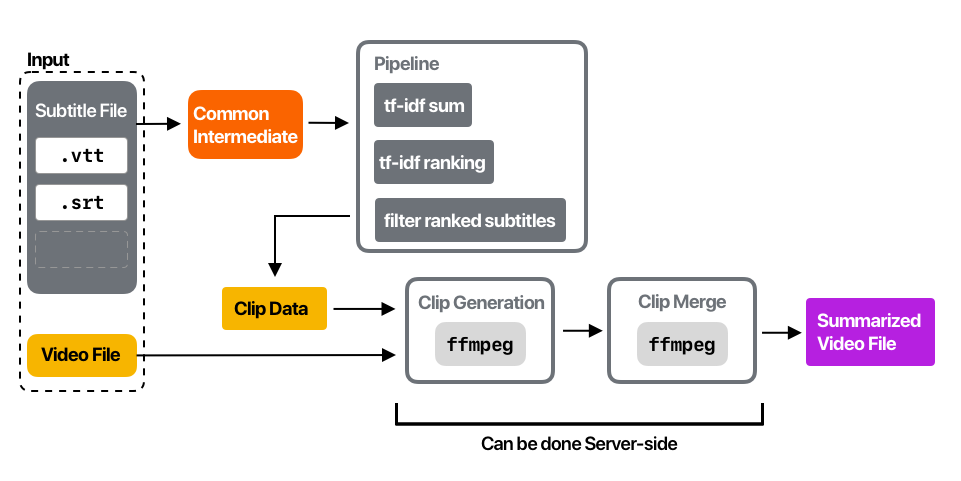
\includegraphics[width=\textwidth, keepaspectratio=true]{Graphic}	
				\caption{Current Pipeline}
				\label{currentpipeline}
		\end{figure}
	\section{Logic}
		This project creates a video summary taking into account multiple video features. The fact that subtitles are ever-present in videos of today especially in long form videos that warrant summarization, significantly eases this task. Academic videos specifically from portals like NPTEL, Coursera and other MOOC platforms make use of lecture transcriptions in order to facilitate learning which can be easily leveraged in order to enable summarization. 
			
		\subsection{Subtitle Parsing}	
			The current implementation leverages these embedded subtitles by supporting both kinds of popular \verb|.srt| and \verb|.vtt| files extracted from the video. Further, auto-generated YouTube captions can also be utilized for the second module.
			
			The first module takes in the subtitle files, (\verb|.srt| and \verb|.vtt|) and parses them into an intermediate file. This ensures that the text learning module can be run independent of the subtitle format. The intermediate incorporates the subtitle entry length, one-indexed subtitle entry (\verb|.srt| includes indices while \verb|.vtt| lacks indices). The subtitle file reading is chunked to efficiently handle large subtitle files and preventing the whole file from loading onto the memory.
			
		\subsection{Text Learning}
			Now the second module is invoked which works on the intermediate file generated by the subtitle parser. Common intermediate file is loaded, then punctuation is stripped. Further common English stop words are removed and the subtitle entry string is lemmatized using a \verb|WordNet Lemmatizer|. Next a tf-idf vectorizer is called upon this data which returns the tf-idf matrix.
			
			Summing the tf-idf matrix across columns gives us a column matrix with one cell for each subtitle entry representing the tf-idf sum of the words in the subtitle.
			
			Since, the parser module also returns the duration of a subtitle, arranging it in descending order and summing up the durations till it exceeds the required length gives the subtitle entries to include in the final output video. 
			
			\subsubsection{Flexibility Parameter}
				Now the concept of a flexibility parameter is introduced. Say, from Figure~\ref{flexparam}, the green entries indicate the initially selected subtitle entries based on the tf-idf sum ranking. 
				
				Based on the value of the flexibility parameter, say \(N\), selected subtitle entries with \(\leq N\) unselected entries in between are also selected.
				
				Setting the parameter to zero generates a summary that's as close as possible to the required length. Whereas, setting the parameter to a large value will include the whole video.
				
				\begin{figure}[ht]
				\centering
					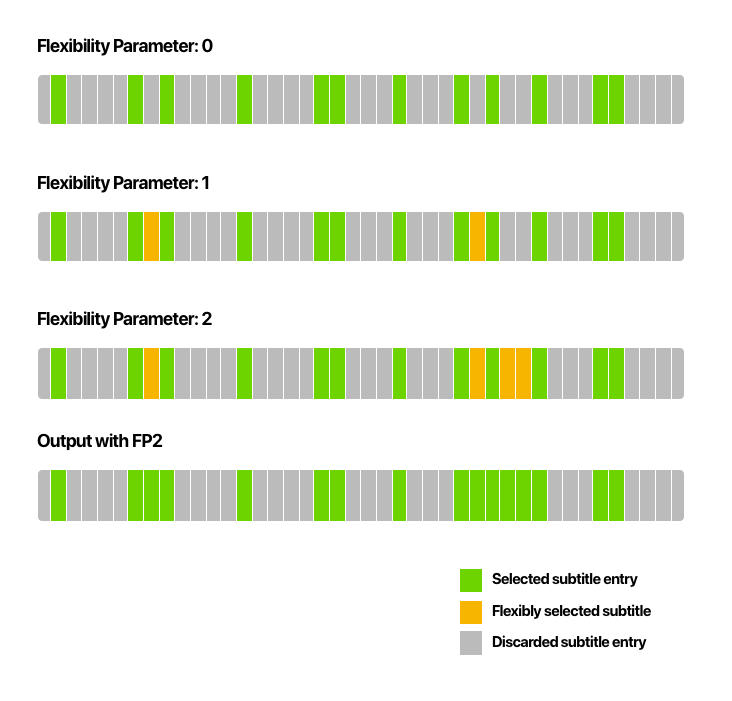
\includegraphics[width=0.8\textwidth, keepaspectratio=true]{Flexibility}	
					\caption{Flexibility Parameter}
					\label{flexparam}
				\end{figure}
				\begin{mdframed}
					\textbf{\underline{Need}}\\
						The concept of flexibility parameter tackles the fundamental idea that if two subtitle entries close by are important then the subtitles between them are important enough to be included in the summary.
						
						This also ensures that the final output is smoother and is not jarring to view. As a result of the flexibility parameter, the final video output becomes longer than the required length.
				\end{mdframed}
			This module creates another intermediate file with the start time, end time and the index of the clips to cut and join to create the summary. 
		
		\subsection{Clip and Summary Creation}	
			Now the final module takes in the intermediate clip data and parses it. It takes in the time stamps and rounds it. The subtitle entries have exact times (down to microseconds) to start showing subtitles and to stop showing the subtitles. The start times are floored down and the stop times are ceiled up. 
			
			
			Next the multiprocessing module calls \verb|ffmpeg| running parallel on the processor of the computer. Finally the created subclips are merged together, again using \verb|ffmpeg| to create the output. \verb|ffmpeg| uses hardware acceleration to encode video streams (For example, h264\_videotoolbox and h265\_videotoolbox are Apple's GPU access API on macOS and \verb|nvenc| for nVidia GPUs).
			
			\begin{mdframed}
				\textbf{\underline{Advantages}}\\
					Since the clip creation and summary generation is running independent as long as the video and the subclip intermediate is available, the initial generation can be done on-device and then the heavy work can be run completely server side leveraging large parallel processing power.
			\end{mdframed}
			
	\section{Results}
	
	The following table shows the compilation of the results after running the code on multiple machines. On a non-parallelized setup using an Nvidia GPU, still gives comparable results when running on parallelized CPU setup.

		\begin{table}[ht]
		\caption{Results}\label{results}
		\vspace{3mm}
\begin{tabular}{|c|c|c|c|c|c|c|}
\hline
S. No              & Video Title                                            & Video Length              & Flex. Param.       & Video Segments      & Quality                & Bitrate                \\ \hline \hline
\multirow{7}{*}{1} & \multirow{7}{3cm}{How to Move the Sun - Stellar Engines} & \multirow{7}{*}{9 m 00 s} & \multirow{5}{*}{2} & \multirow{5}{*}{15} & \multirow{2}{*}{1080p} & \multirow{2}{*}{5094k} \\
                   &                                                        &                           &                    &                     &                        &                        \\ \cline{6-7} 
                   &                                                        &                           &                    &                     & \multirow{3}{*}{480p}  & \multirow{3}{*}{750k}  \\
                   &                                                        &                           &                    &                     &                        &                        \\
                   &                                                        &                           &                    &                     &                        &                        \\ \cline{4-7} 
                   &                                                        &                           & \multirow{2}{*}{3} & \multirow{2}{*}{11} & \multirow{2}{*}{480p}  & \multirow{2}{*}{750k}  \\
                   &                                                        &                           &                    &                     &                        &                        \\ \hline
\end{tabular}\vspace{2mm}

\begin{tabular}{|l|l|l|l|l|l|}
\hline
Encoder            & Bitrate & Text Learning Time (s) & Video gen. Time (s)                   & Time (mins)                   & Final Length                                       \\ \hline \hline
h264\_videotoolbox & default & 2.12 & 687                        & 11 m 27s                       &                                                    \\ \cline{1-4}
default            & default & 2.12 & 1041                       & 17 m 21s                       &                                                    \\ \cline{1-4}
default            & 750k    & 2.12 & 130                        & 2 m 10s                        &                                                    \\ \cline{1-4}
h264\_videotoolbox & default & 2.12 & 83                         & 1 m 23s                        &                                                    \\ \cline{1-4}
h264\_videotoolbox & 750k    & 2.12 & 109                        & 1 m 49s                        &                                                    \\ \cline{1-4}
nvenc (serial)     & 750k     & 2.12 & 109                        & 1m 49s                         & \multirow{-6}{*}{3 m 11 s}                         \\ \hline
nvenc (serial)     & 750k     & 2.12 & \cellcolor[HTML]{67FD9A}78 & \cellcolor[HTML]{67FD9A}1m 18s & \cellcolor[HTML]{67FD9A}                           \\ \cline{1-4}
h264\_videotoolbox & 750k     & 2.12 & \cellcolor[HTML]{67FD9A}61 & \cellcolor[HTML]{67FD9A}1 m 1s & \multirow{-2}{*}{\cellcolor[HTML]{67FD9A}3 m 54 s} \\ \hline
\end{tabular}
\end{table}
		
			\section{Other Modules \& Future Work}
		\begin{itemize}
			\item Implementation of an audio processing pipeline is planned. Since in most educational videos (barring hands-on tutorials), especially with lecture videos, verbal content and worked out content is more important, and visual content importance is lower since it's primarily professors walking. With long length and low resolutions, Deep learning methods fail to distinguish written material on black/whiteboards.
			\item Jarring cuts in video is to be minimized. This can be done by appropriately choosing the parameter \(N\) and implementing crossfade filters and other transitions in \verb|ffmpeg|.
		\end{itemize}

		\begin{figure}[ht]
			\centering
				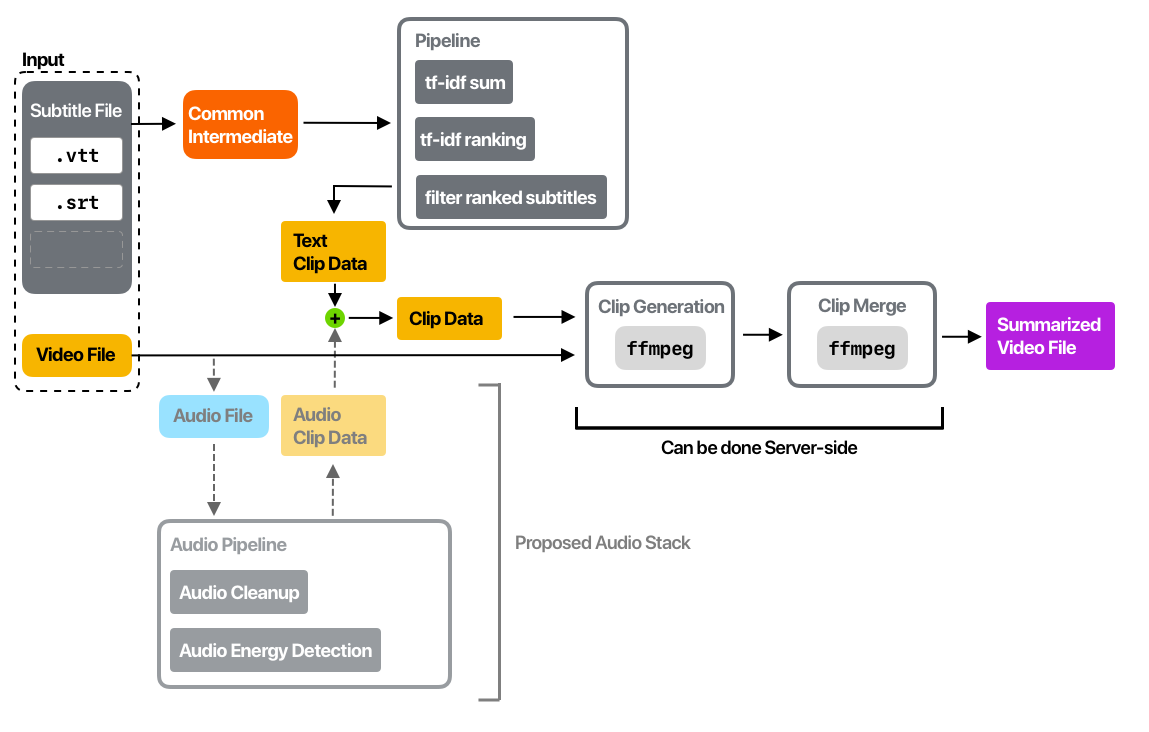
\includegraphics[width=\textwidth, keepaspectratio=true]{Future}	
				\caption{Future Pipeline}
				\label{futurepipeline}
		\end{figure}
	\bibliographystyle{unsrt}
	\bibliography{bibliography}
\end{document}